\documentclass[../main.tex]{subfiles}
\begin{document}
\chapter{Rate Distortion Theory}
Now we discuss information transmission with distortion. \begin{itemize}
    \item Consider compressing an information source with entropy rate $H$ at rate $R < H$ (bad)
    \item By the \textbf{source coding theorem}, $P_e\to 1$ as the block length $n\to \infty$.
    \item Under this this constraint, information must be transmitted with distortion.
    \item What is the best tradeoff then?
\end{itemize}
\centering{Objectives}
\begin{itemize}
    \item Single-letter distortion measures
    \item The rate-distortion function $R(D)$.
    \item The rate-distortion theorem for an iid information source.
\end{itemize}
\section{Single-Letter Distortion Measures}
The setup is as follows: \begin{itemize}
    \item Let $\{X_k,k\geq 1\}$ be an iid information source with generic random variable $X\sim p(x)$ where $|\X|<\infty$ is finite.
    \item Consider a source sequence $\vec x = (x_1,x_2,\dots,x_n)$ and a reproduction sequence $\hat x = (\hat x_1,\dots,\hat x_n).$
    \item The components of $\vec {\hat x}=(\hat x_1,\dots, \hat x_n)$.
    \item The component of $\vec{\hat x}$ take values in \textbf{reproduction alphabet $\hat{\X}$}, where $|\hat{\X}| < \infty$.
    \item In general, $\hat \X$ maybe different from $\X$.
    \item For example, $\vec{\hat x}$ can be a quantized version of $\vec x$.
\end{itemize}
Here comes the definition.
\begin{gbox}{Single-letter distortion measure}
    A single-letter distortion measure is a mapping \[
    d: \X \times \hat \X \to \mathbb{R}^{+}.
    \]
    The value $d(x,\hat x)$ denotes the distortion incurred when a source symbol $x$ is reproduced as $\hat x$. This is intuitive.
\end{gbox}
\begin{gbox}{Average distortion / distortion between sequences}
    The average distortion between a source sequence $\vec x\in \X^n$ and a reproduction sequence $\vec{\hat x}\in \hat \X^n$ induced by a single-letter distortion measure $d$ is defined as \[
    d(\vec x, \vec{\hat x}) = \frac{1}{n}\sum_{i=1}^n d(x_k,\hat x_k)
    \]
\end{gbox}

\begin{pbox}{Examples of a Distortion Measure}
Let $\hat X = X$.
\begin{itemize}
    \item \textbf{Square-error}: \[
    d(x,\hat x = (x-\hat x)^2 
    \] where the source and reproduction RVs are real-valued.
    \item \textbf{Hamming distortion}: \[
    d(x,\hat x) = \begin{cases}
        0\quad \text{if $x=\hat x$}\\
        1 \quad \text{if $x\neq \hat x$}
    \end{cases}.
    \]
\end{itemize}
Let $\hat X$ be an estimate of $X$, \begin{itemize}
    \item If $d$ is the square-error distortion measure, $\mathbb{E} d(X,\hat X)$ is called the mean square error.
    \item $d$ is the Hamming distortion measure, then \[
    \mathbb E d(X,\hat X) = \Pr(X\neq \hat X),
    \]
    which is the probability of error. For a source sequence $\vec x$ and a reproduction sequence $\vec{\hat x}$, the average distortion $d(\vec x,\vec{\hat x})$ gives the frequency of error in $\vec{\hat x}$.
\end{itemize}
\end{pbox}
The distortion measure can be normalized.
\begin{gbox}{Normalization of a Distortion Measure}
    For a distortion measure $d$, for each $x\in X$, let $\hat x^*(x)\in \hat \X$ minimize $d(x,\hat x)$ over all $\hat x\in \hat \X$. A distortion measure is said to be nomral if \[
    c_x := d(x,\hat x^*(x))=0
    \] for all $x\in \X$.
    \begin{remark}
        This says that for normal distortion measure, for each source symbol $x$, there exists some reproduction symbol $\hat x$ such that the distortion between them is $0$.
    \end{remark}
\end{gbox}
\begin{pbox}{Computation of $\hat x^*$}
    Let $d$ be a distortion measure defined by 
    \[
\begin{array}{c|ccc}
d(x, \hat{x}) & \textcolor{red}{\mathbf{a}} & \textcolor{blue}{\mathbf{b}} & c \\
\hline
1 & \underline{\textcolor{red}{2}} & 7 & 5 \\
2 & 4 & \underline{\textcolor{blue}{3}} & 8 \\
\end{array}
\]
Then $\hat x^*(1)=a$ and $\hat x^*(2) = b.$
\end{pbox}
\begin{itemize}
    \item A normal distortion measure is one which allows a source $X$ to be reproduced with zero distortion.
    \item The square-error distortion measure and the Hamming distortion measure are normal distortion measures.
    \item \textbf{To normalize a distortion measure $d$} \[
    \Tilde{d} := d(x,\hat x)-c_x
    \] for all $(x,\hat x) \in \X\times \hat \X$
    \item It suffices to only consider normal distortion measure as we will see.
\end{itemize}
\begin{pbox}{Example of Normalization}
Consider the example above again \[
\begin{array}{c|ccc}
d(x, \hat{x}) & a & b & c \\
\hline
1 & 2 & 7 & 5 \\
2 & 4 & 3 & 8 \\
\end{array}
\]
\[
c_1 = 2, c_2 =3
\]
Then to normalize the measure $d$, we subtract $2$ from the first row and subtract $3$ from the second row to get $\Tilde{d}$:
\[
\begin{array}{c|ccc}
\Tilde{d}(x, \hat{x}) & a & b & c \\
\hline
1 & 0 & 5 & 3 \\
2 & 1 & 0 & 5 \\
\end{array}
\]
\end{pbox}
Let $\hat X$ ne any estimate of $X$ which takes values in $\hat \X$. Then \begin{align*}
    \mathbb{E} d(X,\hat X)&=\sum_x\sum_{\hat x} p(x,\hat x)d(x,\hat x)\\
    &= \sum_x\sum_{\hat x} p(x,\hat x)\Tilde{d}(x,\hat x) + c_x\\
    &= \mathbb{E} \Tilde{d}(X,\hat X) + \sum_x\sum_{\hat x} p(x)p(\hat x|x) c_x\\
    &= \mathbb{E} \Tilde{d}(X,\hat X) + \sum_x p(x)c_x\sum_{\hat x} p(\hat x| x) \\
    &= \mathbb{E} \Tilde{d}(X,\hat X) + \sum_x p(x)c_x\\
    &= \mathbb{E} \Tilde{d}(X,\hat X) + \Delta
\end{align*} where $\Delta := \sum_x p(x)c_x$ is a constant which depends only on $p(x)$ and d but not on the conditional distribution $p(\hat x|x)$
\begin{gbox}{Distortion minimizing point}
    Let $\hat x^*$ minimizes $\mathbb E d(X,\hat x)$ over all $\hat x\in \hat \X$, and define \[
    D_{max} = \mathbb E d(X,\hat x^*)
    \]
    Note: $\hat x^*$ is not the same as $\hat x^*(x)$, and it depends on $p(x)$.
    \begin{itemize}
        \item If we know nothing about a source variable $X$ except for $p(x)$, then $\hat x^*$ is the best estimate of $X$, and $D_{max}$ is the minimum expected distortion between $X$ and a constant estimate of $X$
        \item It's confusing that $D_max$ is called "max", because it should be minimum over $\mathbb E d(X,\hat x)$. We'll see how this makes sense.
        \item Specifically, by taking $\vec{\hat x}^* = (\hat x^*,\dots,\hat x^*)$ to be the reproduction sequence, $D_{max}$ can be asymptotically achived, because by WLLN, \[
        d(\vec X, \vec{\hat x}^*) = \frac{1}{n}\sum_{k=1} d(X_k, \hat x^*) \to \mathbb E d(X,\hat x^*) = D_{max}
        \]
        \item We don't need to consider $D\geq D_{max}$ for the reproduction sequence. This is also why $D_{max}$ is called "D-max" because it's the maximum distortion we would ever care about.
    \end{itemize}
\end{gbox}
\section{The Rate Distortion Function}
We first consider the definition for rate-distortion code. The setup is as follows: 
\begin{itemize}
    \item All the discussions are with respect to an i.i.d. information source $\{X_k,k\geq 1\}$ with generic random variable $X$ and a distortion measure $d.$
\end{itemize}
\begin{gbox}{Rate-Distortion Code}
    An $(n,M)$ rate-distortion code is defined by an encoding function \[
    f:\X^n \to \{1,2,\dots, M\}
    \] and a decoding function \[
    g: \{1,2,\dots, M\} \to \hat X^n
    \]
\end{gbox}
\begin{itemize}
    \item Index set: $\mathcal{I} = \{1,2,\dots,M\}.$
    \item Codewords: the reproduction sequence $g(1),g(2),\dots, g(M)$.
    \item Codebook: the set of all codewords.
    \item 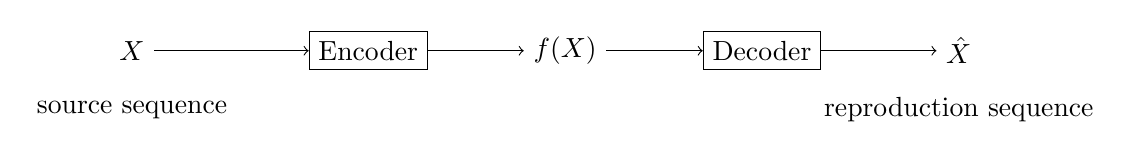
\begin{tikzpicture}[auto, node distance=3cm]

    % Nodes
    \node at (0,0) (X) {$X$};
    \node [below of=X, node distance=0.75cm] {source sequence};
    \node [draw, rectangle, right of=X] (encoder) {Encoder};
    \node [right of=encoder, node distance=2.5cm] (fX) {$f(X)$};
    \node [draw, rectangle, right of=fX, node distance=2.5cm] (decoder) {Decoder};
    \node [right of=decoder, node distance=2.5cm] (Xhat) {$\hat{X}$};
    \node [below of=Xhat, node distance=0.75cm] {reproduction sequence};
    
    % Arrows
    \draw[->] (X) -- (encoder);
    \draw[->] (encoder) -- (fX);
    \draw[->] (fX) -- (decoder);
    \draw[->] (decoder) -- (Xhat);

\end{tikzpicture}
\end{itemize}

\begin{gbox}{Rate of an (n M) rate-distortion code}
    The \textbf{rate} of an $(n,M)$ rate-distortion code is \[
    \frac{1}{n}\log M
    \] in bits per symbol.
\end{gbox}
\begin{gbox}{Achievable rate-distortion pair}
A rate-distortion pair $(R,D)$ is asymptotically achievable if for any $\epsilon > 0$, there exists for sufficiently large $n$ an $(n,M)$ rate-distortion code such that \[
\frac{1}{n}\log M \leq R+\epsilon
\] and \[
\Pr\{d(\vec X, \vec{\hat X}) > D+\epsilon\}\leq \epsilon
\] where $\vec{\hat X} = g(f(\vec X))$.
\begin{remark}
    If $(R,D)$ is achievable, then any $(R',D)$ and $(R,D')$ are also achievable for $R'\geq R$ and $D'\geq D$. i.e. $(R',D')$ are achievable for all $R'\geq R$ and $D'\geq D$.
\end{remark}
\end{gbox}
\begin{gbox}{Rate-distortion region}
A rate-distortion region is the subset of $\mathbb{R}^2$ containing all achievable pairs $(R,D)$.
\end{gbox}
\begin{bbox}{Closedness and Convexity of rate-distortion region}
    The rate-distortion region is closed and convex.
    \begin{proof}
        The closedness follows from the definition of achievability since we had non-strict inequalities. The convexity is proved by a technique called \textit{time-sharing}. 
        \newline
        Time sharing between two codes: one code achieves $(R^{(1)},D^{(1)})$ for $\lambda$ fraction of the time, and the other code achieves $(R^2,D^2)$ for $(1-\lambda)$ fraction of the time.
    \end{proof}
\end{bbox}
\begin{gbox}{Rate-Distortion Function}
    The rate-distortion function $R(D)$ is the minimum of all rates $R$ for a given distortion $D$ such that $(R,D)$ is achievable. 
    \newline
    i.e. we fix $D$ and minimize $R$.
\end{gbox}
\begin{gbox}{Distortion-Rate Function}
    The distortion-rate function $D(R)$ is the minimum of all distortions $D$ for a given rate $R$ such that $(R,D)$ is achievable.
    \newline
    i.e. we fix $R$ and minimize $D$.
\end{gbox}
\begin{remark}
    \begin{itemize}
        \item Most of the time, we will be using $R(D)$ instead of $D(R)$.
        \item If $(R,D)$ is achievable, then $R\geq R(D)$ by definition.
    \end{itemize}
\end{remark}

\begin{bbox}{Properties of rate-distortion function $R(D)$}
\begin{itemize}
    \item $R(D)$ is non-increasing in $D$.
    \item $R(D)$ is convex.
    \item $R(D)=0$ for $D\geq D_{max}$
    \item $R(0)\leq H(X)$
\end{itemize}    
\begin{proof}
    \begin{itemize}
        \item Let $D'\geq D$, $(R(D),D)$ achievable implies that $R(D),D'$ is also achievable. Then $R(D)\geq R(D')$ by definition of $R(D')$.
        \item Follows from the convexity of the rate-distortion region.
        \item $(0, D_{max}$ is achievable implies $R(D_{max})=0$ because $R(D_{max})$ is non-negative. Then $R(D)=0$ for $D\geq D_{max}$ because $R(\cdot)$ is non-increasing.
        \newline
        Note that $R(D_{max})=0$ because there exists a rate-distortion code which has only one codeword - $\hat x^*$, which achieves $D_{max}$ asymptotically.
        \item $(H(X),0)$ is achievable by the source coding theorem. The expected distortion can be made arbitrarily small, since $d$ is normal. Therefore, $R(0)\leq H(X)$ by definition of $R(0)$.
        \newline
        Rigorously, $(H(X),0)$ is achievable because by using a rate no more than $H(X)+\epsilon$, we can describe the source sequence with error probability less than $\epsilon$ by the source coding theorem. Then let the code $\hat X_k = \hat x^*(X_k)$, so that whenever an error does not occur, $d(\vec X, \vec{\hat X})=0$.
    \end{itemize}
\end{proof}
\end{bbox}

\section{The Rate Distortion Theorem}
\begin{gbox}{Information Rate-Distortion Function}
For $D\geq 0$, the information rate-distortion function is defined by \[
R_I(D)=\min_{\hat X: \mathbb{E}d(X,\hat X)\leq D}I(X;\hat X).
\]
\begin{itemize}
    \item The minimization is taken over the set of all transition matrices $p(\hat x|x)$ such that $\mathbb{E}d(X,\hat X)\leq D$:\[
    \{p(\hat x|x):\sum_{x,\hat x}p(x)p(\hat x|x)d(x,\hat x)\leq D\}
    \]
    \item Since this is a topologically compact set (closed and bounded) in $\mathbb{R}^{|\X||\hat \X|}$, and $\I(X,\hat X)$ is a continuous functional of the conditional distribution $p(\hat x|x)$, the minimum value of $\I(X,\hat X)$ can be attained, so $R_I$ is well defined.
    \item Equivalently, the minimization can be taken over the set of all joint distributions $p(x,\hat x)$ with marginal distribution $p(x)$, the given source distribution, such that $\mathbb{E} d(X,\hat X)\leq D.$
    \item Since \[
    \bE \Tilde{d}(X,\hat X) = \bE d(X,\hat X) - \Delta
    \], where $\Delta$ does not depend on $p(\hat x, x),$ we can replace $d$ by $\Tilde{d}$ and $D$ by $D-\Delta$ in the definition of $R_I(D)$ without changing the minimization problem.
    \item Without loss of generality, we can assume $d$ is normal.
\end{itemize}
\end{gbox}
The following theorem is the most important theorem of this chapter.
\begin{bbox}{The Rate-Distortion Theorem}
\[
R(D) = R_I(D)
\]
i.e., the rate-distortion function is actually equal to the information-rate-distortion function.
\end{bbox}
\begin{bbox}{Properties of the information rate-distortion function $R_I(D)$}
    \begin{enumerate}
        \item $R_I(D)$ is non-increasing in $D$.
        \item $R_I(D)$ is convex in $D.$
        \item $R_I(D) = 0$ for $D\geq D_{max}$
        \item $R_I(0) \leq H(X)$
    \end{enumerate}
    \begin{proof}
        \begin{enumerate}
            \item The minimization problem is now over a larger set for larger $D$.
            \item Consider any $D^1, D^2\geq 0$, and $0\leq \lambda\leq 1$. Let $\hat X^i$ achieves $R_I(D^i)$, i.e., \[
                R_I(D^i)=I(X;\hat X^i)
            \] where $\bE d(X,\hat X^i) \leq D^i.$
            \newline
            Let $\hat X^\lambda$ be jointly distributed with $X$ defined by 
            \[
            p_\lambda(\hat x|x)=\lambda p_1(\hat x|x) + (1-\lambda)p_2(\hat x|x).
            \] 
            Then 
            \[
            \bE d(X,\hat X^\lambda) = \lambda \bE d(X,\hat X^1) + (1-\lambda) \bE d(X,\hat X^2)
            \]
            by the linearity of expectation. Then we let \[
            D^\lambda := \lambda D^1 + (1-\lambda) D^2
            \]
            Finally consider \[
            \lambda R_I(D^1) + (1-\lambda) R_i(D^2) = \lambda I(X;\hat X^1) + I(X;\hat X^2) \geq I(X;\hat X^\lambda)
            \] because the mutual information $I(X;Y)$ is a convex functional of $p(y|x)$ for fixed $p(x).$
            \newline
            Lastly, $I(X;\hat X^\lambda)\geq R_I(D^\lambda)$ by definition of $R_I.$

            \item Let $\hat X=\hat x^*$ w.p. $1$ to show that $(0,D_{max})$ is achievable. Then for $R_I(D)\leq I(X;\hat X)=0$ (mutual information with a point mass).

            \item Let $\hat X=\hat x^*(X)$, so that $\bE d(X,\hat X)=0$ since $d$ is normal. Then \[
            R_I(0) \leq I(X;\hat X)\leq H(X)
            \] because mutual information is always less than self-information by information measure diagram.
        \end{enumerate}
    \end{proof}
\end{bbox}
\begin{bbox}{A corollary: stronger properties}
    If $R_1(0) > 0$, then $R_I(D)$ is strictly decreasing for $0\leq D\leq D_{max},$ and the inequality constraint in the definition of $R_I(D)$ can be replaced by an equality constraint.
    \begin{proof}
        Assume by contradiction that $R_I(D')=0$ for some $0\leq D' < D_{max}$, and let $R_I(D')$ be achieved by some $\hat X$. Then 
        \[
        R_I(D')=I(X;\hat X)=0,
        \] meaning $X$ and $\hat X=0$. 
        \newline
        Then note that the estimate $\hat X$ of $X$ does not do a better job than the constant estimate $\hat x^*$ (which minimizes $\bE d(X,\hat x)$ over $\hat x$). 
        Consider \[
        D' \geq \bE d(X,\hat X) = \sum_{x}\sum_{\hat x}p(x,\hat x)d(x,\hat x)
        \]
        By independence, we have \[
        \sum_{x}\sum_{\hat x}p(x,\hat x)d(x,\hat x) = \sum_{x}\sum_{\hat x}p(x)p(\hat x)d(x,\hat x)
        \]
        \[
        =\sum_{\hat x}p(\hat x)\sum_{x}p(x)d(x,\hat x)
        \]
        \[
        =\sum_{\hat x}p(\hat x)\bE d(X,\hat x)
        \]
        \[
        \geq \sum_{\hat x}p(\hat x)\bE d(X,\hat x^*) = D_{max}
        \]
        This is contradiction because we assumed $D' < D_{max}.$
        \newline
        Next we show that $R_I(D)$ must be strictly decreasing for $0 \leq D\leq D_{max}$ because $R_I(0) > 0$, $R_I(D_{max})=0$, and $R_(D)$ is non-increasing and convex. Note that non-strict decreasing messes up with the convexity. (It's helpful draw a curve to visualize.)
        \newline
        Next, show that the inequality constraints in $R_I(D)$ can be replaced by an equality constraint by contradiction.
        Assume by contradiction that $R_I(D)$ is achieved by some $\hat X^*$ such that $\bE d(X,\hat X^*) = D''<D.$ Then \[
        R_I(D'') = \min_{\hat X:\bE d(X,\hat X)\leq D''} I(X;\hat X)\leq I(X;\hat{X^*})= R_I(D),
        \] where the above inequality is true because $I(X;\hat X^*)$ is the minimum over a larger set. This is a contradiction because $R_I(D)$ is strictly decreasing for $0\leq D\leq D_{max}.$
        \newline
        Therefore, $\bE d(X,\hat X^*)$
    \end{proof}
\end{bbox}

\begin{remark}
    $R_I(0)>0$ is not a very strong assumption. In all problems of interest, \[
    R(0) = R_I(0) > 0
    \] because otherwise, $R(D)=0$ for all $D\leq 0$ because $R(D)$ is non-negative and non-increasing. Therefore,\[
    R_I(D) = \min_{\hat X: \bE d(X,\hat X)=D}I(X;\hat X)
    \]
\end{remark}
\begin{pbox}{(Simplest Example) Binary Information Source}
    Let $X$ be a binary random variable with \[
    \Pr\{X=0\}=1-\gamma
    \] and \[
    \Pr\{X=1\} = \gamma.
    \] Let $\hat \X$ be $\{0,1\}=\X$ and $d$ be the Hamming distortion measure.
    
    $\boldsymbol{R_I(D)}$:
    \newline
    First, consider $0\leq \gamma \leq \frac{1}{2}.$ We will show that \[
    R_I(D)=\begin{cases}
        h_b(\gamma) - h_b(D) \quad &\text{if $0\leq D < \gamma$}\\
        0 \quad &\text{if $D \geq \gamma$}
    \end{cases}
    \]
    \begin{proof}
        \begin{enumerate}
            \item Since $\gamma \leq \frac{1}{2}$, $\hat x^* = 0$ and $D_{max}=\bE d(X,0)=\Pr(X=1)=\gamma$.
            \item Consider any $\hat X$ and let $Y=d(X,\hat X).$
            \item $H(X|\hat X)=H(Y|\hat X).$ because given $\hat X$, $X$ and $Y$ can determine each other.
            \newline
            Then for any $\hat X$, such that $\bE d(X,\hat X)\leq D$, where $D< \gamma =D_{max}$, \begin{align*}
                I(X;\hat X) &= H(X)-H(X|\hat X)\\
                &= h_b(\gamma) - H(Y|\hat X)\\
                &\geq h_b(\gamma) - H(Y) \\
                &= h_b(\gamma) - h_b(\Pr(X\neq \hat X))\\
                &\geq h_b(\gamma) - h_b(D),
            \end{align*}
            because $\Pr\{X\neq \hat X\}=\bE d(X,\hat X)\leq D$ and $h_b(a)$ is increasing for $0\leq a\leq \frac{1}{2}.$
            \newline
            Therefore, \begin{align*}
                R_I(D) &= \min_{\hat X:\bE d(X,\hat X)\leq D} I(X;\hat X)\geq h_b(\gamma) - h_n(D).
            \end{align*}
            Now we need to construct $\hat X$ which gives tightness for the above inequalities so that the above bound can be achieved. We need: \begin{itemize}
                \item $Y$ independent of $\hat X$
                \item $P(X\neq \hat X) = D$
            \end{itemize}
            The required $\hat X$ can be constructed by a reverse BSC, i.e. with probability $D,$ $\hat X\neq X$ (Here, $D$ is the cross-over probability). This satisfies the above 2 conditions.
            \newline
            Then let $P(\hat X=0) = \frac{1-\gamma-D}{1-2D}$, and $P(\hat X=1)=\frac{\gamma -D}{1-2D}$.
            \newline
            We can verify that: \[
            P(X=1)=\frac{1-\gamma-D}{1-2D} \times D + \frac{\gamma -D}{1-2D} \times (1-D) = \gamma
            \]
            \item Therefore, we see that for $0\leq \gamma \leq \frac{1}{2},$
            \[
            R_I(D)=\begin{cases}
        h_b(\gamma) - h_b(D) \quad &\text{if $0\leq D < \gamma$}\\
        0 \quad &\text{if $D \geq \gamma = D_{max}$}
    \end{cases}
            \]
            \item Finally, do the same thing to the case where $\frac{1}{2} \leq \gamma \leq 1$ to get \[
            R_I(D)=\begin{cases}
        h_b(\gamma) - h_b(D) \quad &\text{if $0\leq D < \min(\gamma,1-\gamma)$}\\
        0 \quad &\text{if $D \geq \min(\gamma, 1-\gamma)$}
    \end{cases}
            \]
        \end{enumerate}
    \end{proof}
    \begin{remark}
        \begin{itemize}
            \item $R_I(D)$ is the minimum possible mutual information between $X$ and its estimate when the single-letter error probability is $D$.
            \item By the rate-distortion theorem, $R_I(D)$ is also the minimum achievable rate when a single-letter error probability $D$ can be tolerated.
        \end{itemize}
    \end{remark}
\end{pbox}
\begin{remark}
    The source coding theorem is \textbf{NOT} a special case of the rate-distortion theorem. 
    \newline
    In the above example, $R_I(0)=h_b(\gamma)=H(X)$. By the rate-distortion theorem, if $R>H(X)$, the average Hamming distortion (i.e. the error probability per symbol), can be made arbitrarily small. 
    \newline
    However, by the source coding theorem, if $R>H(X)$, the message error probability can be made arbitrarily small, which is a much stronger statement, because the message error probability is small implies that the error probability per symbol is small.
\end{remark}
\section{The "Converse" of the Rate-Distortion Theorem}
In this section, we provide a proof for the "converse" of the rate-distortion theorem.
\begin{bbox}{"Converse" of the Rate-Distortion Theorem}
    For any achievable rate-distortion pair $(R,D)$, $R\geq R_I(D)$
    \begin{proof}
        Let $(R,D)$ be any achievable rate-distortion pair, i.e., for any $\epsilon > 0$, there exists for sufficiently large $n$ an $(n,M)$ code such that \[
        \text{rate of the code} = \frac{1}{n}\log M \leq R+\epsilon
        \] and 
        \[
        \Pr\{d(\vec X, \vec{\hat X}) > D+\epsilon\}\leq \epsilon
        \]
        where $\vec{\hat X}=g(f(\vec X))$
        Then
        \begin{align*}
            n(R+\epsilon) &\geq \log M\\
            &\geq H(f(\vec X))\\
            &\geq H(g(f(\vec X)))\\
            &= H(\vec{\hat X})\\
            &= H(\vec{\hat X}) - H(\vec{\hat X}|\vec X) \quad \text{because $\vec{\hat X}=g(f(\vec X))$}\\
            &= I(\vec{\hat X}; \vec X)\\
            &=H(\vec X) - H(\vec X|\vec{\hat X})\\
            &=\sum_{i=1}^n H(X_k) - \sum_{k=1}^n H(X_k|\vec{\hat X},X_1,X_2,\dots,X_{k-1})\\
            &\text{because the source is iid, chain rule}\\
            &\geq \sum_{k=1}^n H(X_k) - \sum_{k=1}^nH(X_k|\hat X_k)\\
            &=\sum_{k=1}^n I(X_k,\hat X_k)\\
            &\geq \sum_{k=1}^n R_I(\bE d(X_k,\hat X_k))\\
            &= n(\frac{1}{n}\sum_{k=1}^n R_I(\bE d(X_k,\hat X_k)))\\
            &\geq n R_I(\frac{1}{n}\sum_{k=1}^n \bE d(X_k,\hat X_k)) \quad \text{by convexity}\\
            &= n R_I(\bE d(\vec X, \vec{\hat X}))
        \end{align*}
        Now let $d_{\max}=\max_{x,\hat x}d(x,\hat x)$. Then \begin{align*}
            &\bE d(\vec X,\ vec{\hat X}) \\
            &= \bE [d(\vec X, \vec{\hat X})|d(\vec X, \vec{\hat X})>D+\epsilon] \Pr(d(\vec X, \vec{\hat X}) > D+\epsilon)\\
            &+\bE [d(\vec X, \vec{\hat X})|d(\vec X, \vec{\hat X})\leq D+\epsilon] \Pr(d(\vec X, \vec{\hat X}) \leq  D+\epsilon) \\
            &\leq d_{max}\times \epsilon + (D+\epsilon) \times 1\\
            &\to D \quad \text{as $\epsilon \to 0$}
        \end{align*}
        Therefore \begin{align*}
            R+\epsilon &\geq R_I(\bE d(\vec X, \vec{\hat X}))\\
            &\geq R_I(D+(d_{max} + 1)\epsilon)
        \end{align*}
        because $R_I(D)$ is non-increasing in $D.$
        \newline
        Then by convexity of $R_I(D)$, it is continuous in $D$, so by letting $\epsilon \to 0$, we have \begin{align*}
        R &\geq \lim_{\epsilon\to 0}R_I(D+(d_{max}+1)\epsilon)\\
        &= R_I(\lim_{\epsilon\to 0} D+(d_{max}+1)\epsilon) \quad \text{by continuity}\\
        &= R_I(D)
        \end{align*}
    \end{proof}
\end{bbox}
\end{document}